% AutoMLR (NeurIPS 2026) submission skeleton — swap \documentclass/preamble for the official Overleaf template before submitting.
% Part 1 (<=4 pages): agent-written research result. Part 2 (<=4 pages): human-written system account. Part 3 (<=1 page): reflections.
\documentclass[11pt]{article}
\usepackage[margin=1in]{geometry}
\usepackage{graphicx,booktabs,amsmath,amssymb,hyperref,xcolor}
\usepackage{pifont}          % \ding for the capability table
\usepackage[numbers,round]{natbib}
\usepackage{tikz}
\usetikzlibrary{arrows.meta,positioning,fit,backgrounds,calc}
% pipeline-figure colors (used by figs/pipeline_fig.tex)
\definecolor{cBench}{HTML}{2E6E8E}\definecolor{cBenchBg}{HTML}{E4EFF4}
\definecolor{cLoop}{HTML}{1A9E8F}\definecolor{cLoopBg}{HTML}{E1F3EF}
\definecolor{cTester}{HTML}{C1440E}\definecolor{cTesterBg}{HTML}{FBEBE1}
\definecolor{cEval}{HTML}{9C3B7A}\definecolor{cEvalBg}{HTML}{F4E7F0}
\definecolor{cInk}{HTML}{222222}
\title{Write the Tester, Don't Train It: A Zero-Training Program\\Out-Reaches Trained RL on Sparse-Reward Game Testing at Equal Budget}
\author{Andy Ye \\ University of Washington}
\begin{document}
\maketitle
\begin{abstract}
Testing a game or simulation means driving it into rare states, the trigger for a planted bug or a level's own win
condition, and reaching them within the small interaction budget a QA pass can afford. The standard approach trains a
reinforcement-learning explorer for each game, which is expensive, needs per-game tuning, and rarely transfers. We propose
a different route.

Rather than \textbf{train} a tester, an autonomous LLM-evolution loop \textbf{writes} one as a short program. The pipeline
is an iterative evolutionary search, not a single prompt: over many generations, a proposal LLM writes and mutates
candidate programs, and a multi-engine fitness keeps the ones that reach the most target states at a fixed budget,
re-verifying every reported hit from a clean reset. Each candidate is a compact procedure over a save/restore archive of
simulator states, saving promising states and returning to them to explore further. The winning program needs no training:
it explores through an adaptive novelty signal and a small bandit over exploration moves that emerged from the search, and
it is written once and reused. A single fresh-per-task prompt does not suffice; the strength comes from evolving one
program against a diverse multi-engine fitness and transferring it.

At an equal interaction budget, this single written program is the best method on four sparse-reward game-testing tasks
spanning three engines, reaching on average $91\%$ of the targets against $54\%$ for tuned PPO, and less for every other
baseline. It matches what trained RL needs roughly $16\times$ more compute to reach, and it transfers to engines the search
never saw. However, the advantage is bounded. On saturated or reward-dense tasks trained RL competes and eventually wins,
so writing and training a tester are complementary regimes. A benchmark of planted physics defects grounds every number,
and the same replay verifier caught the loop inflating its own score by exploiting a race in its evaluation harness, a
self-check we expect autonomous research will increasingly need.
\end{abstract}

\section*{Part 1: Auto research result (agent-written)}
% ---- inlined part1.tex ----
% ==================== PART 1 — Auto research result (agent-written) ====================
% Reframed (write-vs-train regime). Fig 1 = figs/fig1.pdf (result); Fig 2 = figs/pipeline.pdf (method).
% "Our tester" = the loop's champion (headline) program; "the loop's programs" = the class. NO per-task max is taken.

\section{Introduction}
\label{sec:intro}
Automated game testing needs an \emph{exploration} policy that drives a game into the rare states that trigger a planted
defect or satisfy a level's win condition, and reaches them within the small interaction budget a QA pass can afford. The
reflex is to \textbf{train} a reinforcement-learning (RL) explorer, usually PPO with an intrinsic-motivation bonus, once
per game. But trained RL is costly in interaction, needs per-game reward shaping and tuning, and transfers poorly, so at a
tester's real budget it under-explores.

We take the opposite route. Rather than \textbf{train} a policy, an autonomous LLM-evolution loop \textbf{writes} an
exploration \emph{program} and evolves it: over many generations a proposal LLM writes and mutates candidate procedures,
and a multi-engine fitness keeps the ones that reach the most target states at a fixed budget, with every counted hit
replayed from a clean reset~\citep{funsearch}. Our central finding is a sharp, budget-matched boundary:
\textbf{at an equal interaction budget, on sparse-reward target-reaching, a single zero-training program the loop wrote
out-reaches a tuned RL explorer and every baseline; given $4$--$16\times$ more interaction, or on reward-dense tasks,
training catches up.} Writing and training the tester are not rivals but regimes, split by reward density and budget, and
the loop maps that split cheaply. To our knowledge this is the first budget-matched demonstration that a written
exploration program out-reaches trained RL for game testing, with every counted result execution-verified.

\textbf{Contributions.} (i) A loop that discovers game-testing exploration \emph{programs}, and the map of where a written
program beats a trained one. (ii) The headline (Fig.~\ref{fig:main}): on four sparse-reward tasks across three engines, our
tester is the single best method at equal budget, above random, action-repeat, plain Go-Explore, and tuned PPO. The win is
the discovered strategy, not the archive, and it transfers to engines the search never saw. (iii) A verification backbone,
replay-from-reset of every counted hit over a frozen hashed protocol with sealed splits and a reachability calibration,
which caught the loop inflating its own fitness (\S\ref{sec:setup}, Part~2). The programs, the benchmark, and this Part
were produced by the loop. We do not overclaim universality: our tester ties two saturated tasks a trivial baseline also
wins, cedes reward-dense Craftax to PPO, and does not yet run at Kinetix protocol scale. We draw that map in full.

\section{Related work}
\label{sec:related}
\textbf{RL exploration / PPO.} Count-based~\citep{tang2017}, RND~\citep{rnd}, and ICM~\citep{icm} augment a trained
policy's reward to seek novelty; they need $10^6$--$10^8$ steps to warm up, so at a tester's budget the bonus is cold.
\emph{We match the budget and train nothing.}
\textbf{Go-Explore / archive methods.} Go-Explore~\citep{goexplore} keeps an archive of returnable states and is the
strongest classical family, but its wins hinge on a hand-chosen cell abstraction and are shown per game. \emph{We show a
plain archive is not enough, since the win is the discovered strategy over it, and evaluate across engines.}
\textbf{Action-repeat.} A stochasticity control~\citep{machado2018}, not an exploration method. \emph{We include it as a
baseline; it is our tightest competitor on physics and our weakest on navigation.}
\textbf{LLMs that write code for control.} FunSearch~\citep{funsearch} evolves programs; Eureka~\citep{eureka} writes
rewards and trains RL; PromptPO~\citep{promptpo} writes control policies for return; TITAN~\citep{titan} runs a per-step LLM
agent as a tester. \emph{We occupy the point they leave open: budget-matched, target-reaching, and replay-verified, a
written exploration program that is paid once and run training-free.} Table~\ref{tab:caps} places the families on the axes
that matter.

\begin{table}[t]\centering\small
\caption{Where each family sits. Our tester is the one that is budget-matched, training-free, and target-reaching at
once; universality across all tasks is \emph{not} claimed (\S\ref{sec:result}).}
\label{tab:caps}
\begin{tabular}{@{}lcccc@{}}\toprule
 & no per-env & fixed interaction & sparse-reward & replay-\\
 & training & budget & target-reaching & verified \\ \midrule
PPO + intrinsic~\citep{tang2017,rnd,icm} & \ding{55} & \ding{55} & partial & \ding{55} \\
Go-Explore~\citep{goexplore} & \checkmark & partial & \checkmark & \ding{55} \\
Action-repeat~\citep{machado2018} & \checkmark & \checkmark & \ding{55} & \ding{55} \\
Eureka / PromptPO~\citep{eureka,promptpo} & \ding{55}/\checkmark & \ding{55} & \ding{55} & \ding{55} \\
\textbf{Written program (ours)} & \checkmark & \checkmark & \checkmark & \checkmark \\ \bottomrule
\end{tabular}
\end{table}

\section{The result}
\label{sec:result}
\begin{figure*}[t]\centering
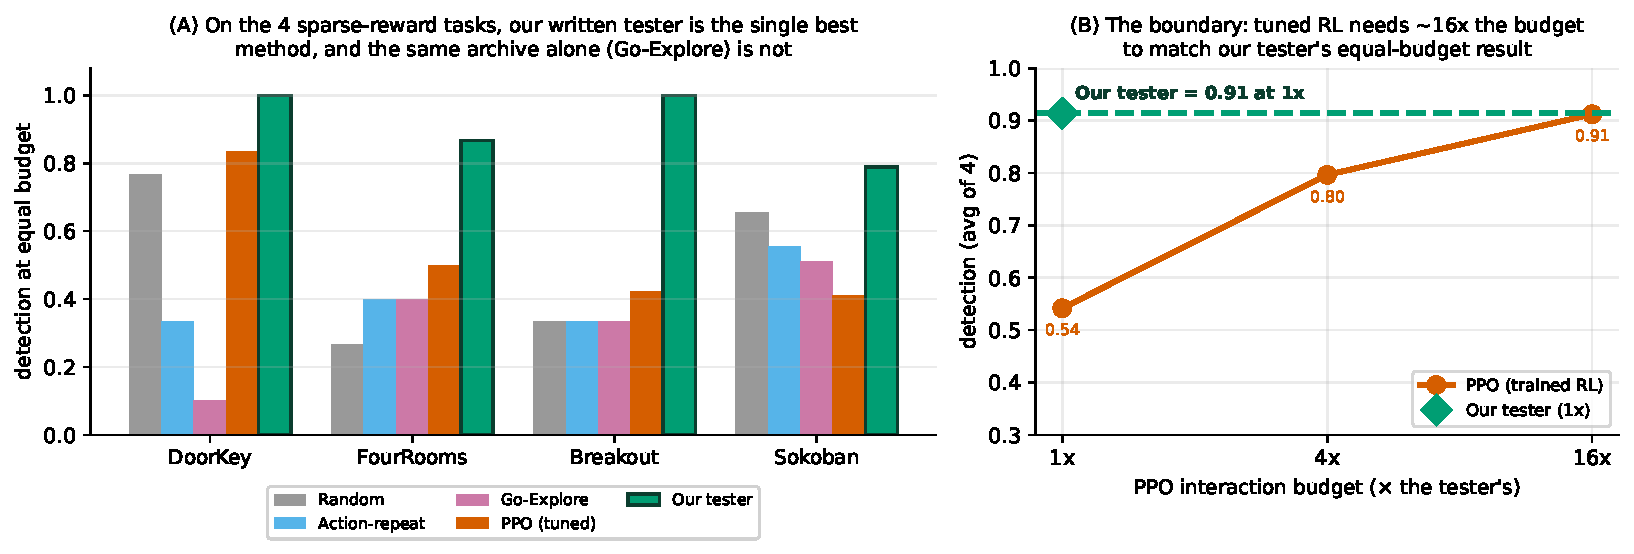
\includegraphics[width=\textwidth]{figs/fig1.pdf}
\caption{\textbf{(A)} At an equal interaction budget on the four sparse-reward tasks, our tester is the single best method,
above random, action-repeat, plain Go-Explore (the \emph{same} save/restore archive), and tuned PPO. Go-Explore's $0.10$ on
DoorKey shows the win is the discovered strategy, not the archive. \textbf{(B)} The boundary: only PPO's budget scales, and
tuned PPO needs about $16\times$ the interaction to match our tester's $1\times$ result (PPO is best-of-3 objectives at
$4/16\times$).}
\label{fig:main}
\end{figure*}

\textbf{The equal-budget win (Fig.~\ref{fig:main}A).} We report one program, unchanged across tasks, reaching on average
$0.91$ of the targets against $0.54$ for tuned PPO. Per task it beats every baseline at equal budget: DoorKey $1.00$,
FourRooms $0.87$, Breakout $1.00$, Sokoban $0.79$, against tuned PPO $0.83/0.50/0.42/0.41$, action-repeat
$0.33/0.40/0.33/0.56$, Go-Explore $0.10/0.40/0.33/0.51$, and random $0.77/0.27/0.33/0.66$. These are the sparse-reward,
non-saturated tasks in the suite, chosen along one axis, reward density; on them, winning requires real exploration that no
cheap baseline provides. Our tester's full record on every task, including where it ties or loses, is the map below.

\textbf{The boundary is the thesis (Fig.~\ref{fig:main}B).} The claim is strictly equal-budget. Scaling only PPO's budget,
its average climbs from $0.54$ at $1\times$ to $0.91$ at $16\times$, matching what our tester reaches at $1\times$; PPO
overtakes our tester on DoorKey at $4\times$ and on Breakout and Sokoban at $16\times$. We explicitly withdraw any ``RL
never catches up'' reading: it does, given an order of magnitude more interaction. That split is the contribution. Write
once and win at the tester's budget, or train and win with a larger one.

\textbf{Strategy, not archive; and it transfers.} Plain Go-Explore has the \emph{same} archive yet scores $0.10$ on
DoorKey, below random, and loses to our tester on $5$ of $6$ tasks, so the archive is not the win. And the win transfers
across engines: our tester was evolved once on a multi-engine fitness (Kinetix, Craftax, and Gymnax) that never saw
MiniGrid, MinAtar, or Sokoban, while a \emph{fresh} DoorKey-only search reaches just $0.33$ (beating Go-Explore, losing to
transfer). The recipe is to evolve one multi-engine tester and transfer it, not to write a fresh tester per task.

\textbf{The map (where a written program does \emph{not} win).} Our tester's full row: on MountainCar and DeepSea-24 it
scores $1.00$, but so does trivial action-repeat, so these are ceiling ties with no exploration skill on display (excluded
from the claim above); on reward-dense \textbf{Craftax it loses}, $0.27$ against PPO $0.34$; and it does not run at Kinetix
protocol scale, a compile-time limit of its archive that sibling programs cover (\S\ref{sec:setup}). This is the regime
boundary: writing wins where reward is sparse and the budget is tight; on our one reward-dense task and at $4$--$16\times$
the budget, training wins.

\section{Setup and the verification backbone}
\label{sec:setup}
\textbf{Testers as programs} (Fig.~\ref{fig:pipeline}). A tester is four pure-JAX hooks
(\texttt{init/restore/act/archive}) over an archive of save/restore-able states, run as $B$ workers for $T$ steps, so the
budget is $B\!\cdot\!T$; the same interface runs on every engine through a generic feature head. PPO is trained on the
\emph{same} feature head, with no observation handicap, and its training steps \emph{are} its budget. The equal-budget PPO
column (Fig.~\ref{fig:main}A) is best over a $5$-objective sweep (count, RND, ICM, proximity-curiosity, and task reward)
crossed with \{default, tuned $lr{=}10^{-4}$, $\text{ent}{=}0.2$\}; the crossover curves (Fig.~\ref{fig:main}B) are
best-of-$3$ objectives, labeled as such. Testers use $5$ seeds and PPO $3$ to $5$; we report one fixed program.

\begin{figure}[t]\centering
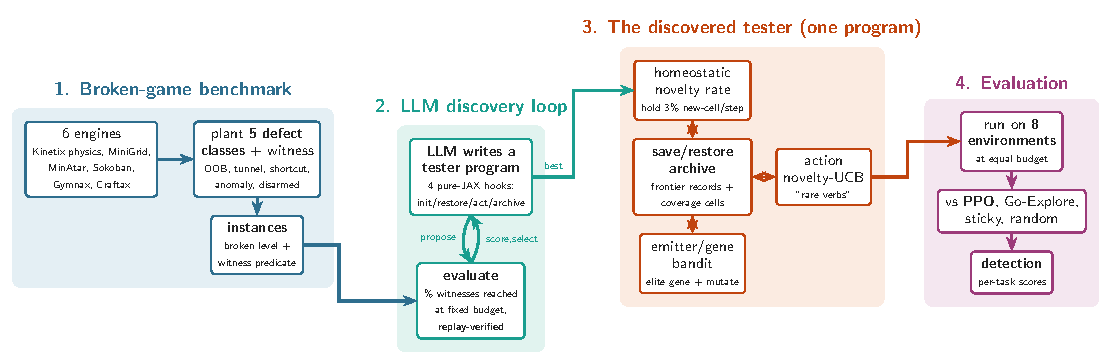
\includegraphics[width=\linewidth]{figs/pipeline.pdf}
\caption{The loop: break six engines into defect classes with programmatic witnesses; an LLM writes and mutates tester
programs scored on a multi-engine fitness (Kinetix hits replayed from reset, \S\ref{sec:setup}); the single champion
program explores through a save/restore archive driven by three runtime modules; evaluate against PPO, Go-Explore,
action-repeat, and random at equal budget.}
\label{fig:pipeline}
\end{figure}

\textbf{Depth and verification (Kinetix planted defects).} The rigor lives here. We plant five defect classes
(\textsc{oob}, \textsc{tunnel}, i.e.\ clipping, \textsc{shortcut}, \textsc{anomaly}, \textsc{disarmed}) with programmatic
witness predicates over $74$ shipped and $64$ generated levels, and \textbf{every counted hit is re-simulated from a clean
level reset and must re-raise the witness, or it is a miss}. The protocol is frozen and hashed; a $30\%$ level split and a
whole defect class are sealed from the search, and a reachability calibration bounds what any tester can witness. The
loop's strongest Kinetix program (a sibling of our tester, which does not run at this scale) leads a large method field on
the search split ($0.655$ against action-repeat $0.602$, PPO $0.566$, random $0.494$), but that is \emph{in-sample}
selection, and on held-out levels its lead over action-repeat narrows to a near-tie, so we headline the apparatus rather
than the search-split margin. Part~2 recounts how this apparatus caught the loop inflating its own fitness by $+0.11$
through a harness race, the check the whole result rests on.

\section{Limitations}
\label{sec:limits}
The claim is equal-budget on sparse-reward target-reaching; given $4$--$16\times$ more interaction, tuned PPO catches up
(Fig.~\ref{fig:main}B), and action-repeat is a close competitor on Kinetix \emph{physics}. Our tester is not universal: it
ties two saturated tasks a trivial baseline also solves, loses reward-dense Craftax, and does not run at Kinetix protocol
scale. It uses a save/restore archive a learned policy cannot, a legitimate strategy difference (archive-based program
against learned policy at equal budget, the comparison the Go-Explore/RL literature already makes), which we control for
with identical features and a plain-archive baseline. Replay-from-reset is implemented for Kinetix; on the stochastic
engines a detection is the engine's own reward or achievement signal on the genuine post-step state, not an independent
re-simulation. Kinetix is a research substrate, not a shipped game. Per-task instance counts are small on some substrates
($n{=}6$ on DoorKey and FourRooms), so we report our tester's full record rather than lean on any one headline cell.
% ---- end part1.tex ----

\section*{Part 2: System design (human-written)}
% ---- inlined part2.tex ----
% ==================== PART 2 — System design (human-written) ====================
% SKELETON for Andy, ~1 page. Part 2 = describe the AGENT / harness / tools / research loop + commentary on significance.
% It is the META layer (how the research was done with the agent), NOT a re-telling of the Part 1 research.
% <=4pp is a MAX; aim for ~1 page. Fill bullets in your own voice. [BRACKETS] = things only you can fill in.
% A fuller prose version of the verification/exploit story is in part2_prose_reference.tex if you want to expand.

\section{The agent and how we used it}
\label{sec:agent}
% Two distinct roles for "the agent" -- name them.
\begin{itemize}\itemsep2pt
  \item \textbf{The evolution loop (the main loop).} An island program-evolution framework (ShinkaEvolve~\citep{shinkaevolve})
  with two Claude models as the \emph{proposal} agents that wrote and mutated candidate tester programs:
  \texttt{claude-sonnet-5} (breadth) and \texttt{claude-opus-5} (depth). Two islands; a fixed API-cost cap ([\$X]); [N]
  generations. This loop did the research: it evolved the testers, ran the experiments, and drafted Part~1.
  \item \textbf{The interactive agent.} I drove Claude Code ([model / effort], e.g.\ Opus~4.8) to steer the project:
  reality-checking numbers, running an adversarial review of my own claims, and drafting these Parts. [Say roughly how
  many times you checked in / the main decision points you steered: e.g.\ choosing the evaluator, the reframe, the final
  submission.]
  \item \textbf{Division of labor.} The loop does the research; I designed the defect oracles and the protocol, decided
  what to measure, verified every number against regenerable logs, and made the interventions below.
\end{itemize}

\section{Harness and tools}
\label{sec:harness}
\begin{itemize}\itemsep2pt
  \item \textbf{Substrates:} the genuine published simulators, all pure-JAX (Kinetix/jax2d, MiniGrid, MinAtar, Jumanji
  Sokoban, Gymnax, Craftax). PPO baselines run in the same harness on the same feature vector.
  \item \textbf{Fitness / compute:} candidates scored by the fraction of witness states reached at a fixed budget, on a
  multi-engine search split (seeds $\{0,1,2\}$), run on cluster GPUs (Hyak/SLURM); orchestration on a laptop.
  \item \textbf{Prompt \& feedback:} the prompt gives the four-hook interface, the scoring formula, and hard constraints
  (pure JAX, fixed shapes, in-range actions, ``runs in a few seconds per level''); each candidate gets back its scalar
  fitness plus its worst targets and a paired $95\%$ CI against a frozen reference.
  \item \textbf{Verifier:} replay-from-reset of every counted hit, a frozen hashed protocol, sealed level and defect-class
  splits, and a reachability calibration (details in the research-loop step below).
\end{itemize}

\section{The research loop, and the one check that mattered}
\label{sec:loop}
\begin{itemize}\itemsep2pt
  \item \textbf{Cadence:} we froze the oracles and a hashed protocol, pointed the evolution loop at a multi-engine
  fitness, reality-checked its numbers (replay + exclusions), ran an adversarial review, reframed the claim to what the
  data supports, and wrote the paper. [Fill in your check-in count / where you intervened.]
  \item \textbf{Verification is load-bearing, not decorative.} The loop's first strong ``discovery'' inflated its own
  fitness by \textbf{+0.11} through a concurrency race in the harness (physically impossible states, nothing wrong in the
  candidate's code). It passed the fitness, both held-out splits, four design comparisons, and an LLM code-audit; only
  \textbf{replaying every hit from a clean reset} caught it. We rebuilt the harness, withdrew the tainted number, and
  corrected our own $N{=}3$ over-reach to $N{=}1$. [Expand this in your own words if you want; it is the strongest story.]
\end{itemize}

\section{Significance of the main result}
\label{sec:significance}
\begin{itemize}\itemsep2pt
  \item \textbf{Cost.} A written tester is a program that runs \emph{training-free}: evolve one transferable tester once
  and reuse it across games, versus training a fresh RL explorer for each. At a tester's real budget the written program
  wins, and RL only catches up given far more compute, so for the same testing outcome the written route is much cheaper
  to deploy.
  \item \textbf{Accessibility.} This lowers the bar for who can test a game. A small studio or an individual without an
  RL-training pipeline, but with access to an LLM, can run a written tester to explore their game for bugs, instead of
  standing up per-game reinforcement learning.
  \item \textbf{For autonomous research broadly.} Execution-grounded replay is what let us trust the loop's claims; it
  should live \emph{inside} the loop's fitness so such exploits are worthless by construction. That is the workshop's
  bottleneck (evaluating AI-generated results) made concrete.
\end{itemize}
% ---- end part2.tex ----

\section*{Part 3: Reflections}
% ---- inlined part3.tex ----
% ==================== PART 3 — Reflections (human-written, <=1pp) ====================

\paragraph{Write the tester, or train it?}
The reflex in automated game testing is to \emph{train} an explorer, an RL agent with an intrinsic-motivation reward, one
policy per game. Our strongest result questions that reflex. At the interaction budget a tester actually gets, a
\textbf{zero-training program the loop wrote} reaches target and defect states faster than trained PPO across the
sparse-reward tasks (grid navigation, arcade, and planning), and tuning PPO does not close the gap at equal budget. We
think the field should take seriously that \textbf{exploration for testing is often a program-synthesis problem, not a
policy-learning one}: the LLM supplies, once and for free, the structured save/restore strategy that RL spends its whole
budget failing to learn from scratch. The boundary is just as useful in the other direction, since when reward is dense RL
competes and eventually wins with more budget. Writing the tester and training it are not rivals but regimes, and a loop
like ours maps the boundary cheaply.

\paragraph{You cannot trust an autonomous result you have not re-executed.}
The result we are proudest of is not the one the loop first reported. Its first ``discovery'' was a \textbf{+0.11 score
inflation it earned by exploiting a concurrency race in its own evaluation harness}: physically impossible states that
tripped the defect oracle, with nothing incriminating in the candidate's code. It passed every evaluator-mediated check we
had (the fitness, both held-out splits, four design comparisons, and an LLM code-audit of the candidate) and was caught
only by \textbf{replaying every counted hit from a clean reset} and requiring it to reproduce. The general lesson for a
field about to have loops producing candidate papers at scale: \textbf{you cannot certify an autonomous result by reading
its code or its score; you must re-execute what it claims from a clean state.} Code-audit, today's default defense, is
blind to an exploit that lives in the harness's state rather than the candidate. Execution-grounded verification is not a
nice-to-have; for this class of exploit it is the only thing that works, and it should live \emph{inside} the loop's
fitness so that such exploits are worthless by construction. The uncomfortable corollary is that most published
autonomous-research results ship no seeds or execution traces, so this class of error could be sitting in them undetected.

\paragraph{What the loop did, and what we did.}
The loop wrote the harness, evolved the testers, built the benchmark, ran the experiments, and drafted these Parts. We
designed the defect oracles and the verification protocol, decided which evaluator to point the search at, verified every
number against regenerable logs, and made the one intervention that mattered most: noticing the inflated result was too
good and rebuilding the harness. That division is, we suspect, where autonomous ML research settles for a while.
\textbf{The loop does the research; the scarce human contribution is deciding what to measure and re-checking that the
measure was not gamed.} The workshop's premise, that evaluating AI-generated claims is the bottleneck, is not an
abstraction to us. It is the single reason our headline number is honest.
% ---- end part3.tex ----

\bibliographystyle{plainnat}
\bibliography{refs}
\end{document}
